\documentclass{book}
\usepackage[a4paper,top=2.5cm,bottom=2.5cm,left=2.5cm,right=2.5cm]{geometry}
\usepackage{makeidx}
\usepackage{natbib}
\usepackage{graphicx}
\usepackage{multicol}
\usepackage{float}
\usepackage{listings}
\usepackage{color}
\usepackage{ifthen}
\usepackage[table]{xcolor}
\usepackage{textcomp}
\usepackage{alltt}
\usepackage{ifpdf}
\ifpdf
\usepackage[pdftex,
            pagebackref=true,
            colorlinks=true,
            linkcolor=blue,
            unicode
           ]{hyperref}
\else
\usepackage[ps2pdf,
            pagebackref=true,
            colorlinks=true,
            linkcolor=blue,
            unicode
           ]{hyperref}
\usepackage{pspicture}
\fi
\usepackage[utf8]{inputenc}
\usepackage{mathptmx}
\usepackage[scaled=.90]{helvet}
\usepackage{courier}
\usepackage{sectsty}
\usepackage{amssymb}
\usepackage[titles]{tocloft}
\usepackage{doxygen}
\lstset{language=C++,inputencoding=utf8,basicstyle=\footnotesize,breaklines=true,breakatwhitespace=true,tabsize=4,numbers=left }
\makeindex
\setcounter{tocdepth}{3}
\renewcommand{\footrulewidth}{0.4pt}
\renewcommand{\familydefault}{\sfdefault}
\hfuzz=15pt
\setlength{\emergencystretch}{15pt}
\hbadness=750
\tolerance=750
\begin{document}
\hypersetup{pageanchor=false,citecolor=blue}
\begin{titlepage}
\vspace*{7cm}
\begin{center}
{\Large Solar Panel Tracker \\[1ex]\large 1.\-0 }\\
\vspace*{1cm}
{\large Generated by Doxygen 1.8.2}\\
\vspace*{0.5cm}
{\small Wed Aug 22 2012 16:40:41}\\
\end{center}
\end{titlepage}
\clearemptydoublepage
\pagenumbering{roman}
\tableofcontents
\clearemptydoublepage
\pagenumbering{arabic}
\hypersetup{pageanchor=true,citecolor=blue}
\chapter{Namespace Index}
\section{Packages}
Here are the packages with brief descriptions (if available)\-:\begin{DoxyCompactList}
\item\contentsline{section}{\hyperlink{namespacegui}{gui} }{\pageref{namespacegui}}{}
\item\contentsline{section}{\hyperlink{namespacelauncher}{launcher} }{\pageref{namespacelauncher}}{}
\item\contentsline{section}{\hyperlink{namespacetiny26}{tiny26} }{\pageref{namespacetiny26}}{}
\end{DoxyCompactList}

\chapter{Hierarchical Index}
\section{Class Hierarchy}
This inheritance list is sorted roughly, but not completely, alphabetically\-:\begin{DoxyCompactList}
\item App\begin{DoxyCompactList}
\item \contentsline{section}{gui.\-G\-U\-I\-\_\-\-Launcher}{\pageref{classgui_1_1_g_u_i___launcher}}{}
\end{DoxyCompactList}
\item Frame\begin{DoxyCompactList}
\item \contentsline{section}{gui.\-Motor\-G\-U\-I}{\pageref{classgui_1_1_motor_g_u_i}}{}
\end{DoxyCompactList}
\item Py\-Command\-Event\begin{DoxyCompactList}
\item \contentsline{section}{tiny26.\-Solar\-Event}{\pageref{classtiny26_1_1_solar_event}}{}
\end{DoxyCompactList}
\item \contentsline{section}{tiny26.\-U\-S\-B\-\_\-\-Interface}{\pageref{classtiny26_1_1_u_s_b___interface}}{}
\item Thread\begin{DoxyCompactList}
\item \contentsline{section}{tiny26.\-Solar\-Tracking\-Thread}{\pageref{classtiny26_1_1_solar_tracking_thread}}{}
\end{DoxyCompactList}
\end{DoxyCompactList}

\chapter{Class Index}
\section{Class List}
Here are the classes, structs, unions and interfaces with brief descriptions\-:\begin{DoxyCompactList}
\item\contentsline{section}{\hyperlink{classgui_1_1_g_u_i___launcher}{gui.\-G\-U\-I\-\_\-\-Launcher} \\*Abstracts away the creation of the \hyperlink{classgui_1_1_motor_g_u_i}{Motor\-G\-U\-I} and launches it in the default constructor }{\pageref{classgui_1_1_g_u_i___launcher}}{}
\item\contentsline{section}{\hyperlink{classgui_1_1_motor_g_u_i}{gui.\-Motor\-G\-U\-I} \\*Defines the main frame for the G\-U\-I }{\pageref{classgui_1_1_motor_g_u_i}}{}
\item\contentsline{section}{\hyperlink{classtiny26_1_1_solar_event}{tiny26.\-Solar\-Event} \\*Event class that allows a background thread to send messages to G\-U\-I to tell it to update itself }{\pageref{classtiny26_1_1_solar_event}}{}
\item\contentsline{section}{\hyperlink{classtiny26_1_1_solar_tracking_thread}{tiny26.\-Solar\-Tracking\-Thread} \\*Contains the definition for the background thread that polls the A\-D\-C input from the solar panel and sends that value to the G\-U\-I to be displayed to the user }{\pageref{classtiny26_1_1_solar_tracking_thread}}{}
\item\contentsline{section}{\hyperlink{classtiny26_1_1_u_s_b___interface}{tiny26.\-U\-S\-B\-\_\-\-Interface} \\*The usb interface for the O\-S\-Uisp2 and the Tiny261 is contained in this class }{\pageref{classtiny26_1_1_u_s_b___interface}}{}
\end{DoxyCompactList}

\chapter{Namespace Documentation}
\hypertarget{namespacegui}{\section{gui Namespace Reference}
\label{namespacegui}\index{gui@{gui}}
}
\subsection*{Classes}
\begin{DoxyCompactItemize}
\item 
class \hyperlink{classgui_1_1_motor_g_u_i}{Motor\-G\-U\-I}
\begin{DoxyCompactList}\small\item\em Defines the main frame for the G\-U\-I. \end{DoxyCompactList}\item 
class \hyperlink{classgui_1_1_g_u_i___launcher}{G\-U\-I\-\_\-\-Launcher}
\begin{DoxyCompactList}\small\item\em Abstracts away the creation of the \hyperlink{classgui_1_1_motor_g_u_i}{Motor\-G\-U\-I} and launches it in the default constructor. \end{DoxyCompactList}\end{DoxyCompactItemize}


\subsection{Detailed Description}
\begin{DoxyVerb}Defines the GUI that abstracts away the connection with the OSUisp2 and Tiny261
Created on Aug 13, 2012

@author: Robert L. Phillips III
@version: 1.0

@section DEPENDENCIES
    -  wxPython
          The GUI is generated using the third party library wxPython.  All documentation
          for the wxPython library can be found at wxpython.org.
          
    -  tiny26
          Contains the libraries necessary for the GUI to establish a connection to the
          Tiny26 and send commands to it.
          
    -  time
          Contains the sleep function, which is needed to block certain threads for a certain
          amount of time
\end{DoxyVerb}
 
\hypertarget{namespacelauncher}{\section{launcher Namespace Reference}
\label{namespacelauncher}\index{launcher@{launcher}}
}
\subsection*{Variables}
\begin{DoxyCompactItemize}
\item 
\hypertarget{namespacelauncher_ae89ee08b571448a6c7d24b325e6c4c15}{tuple \hyperlink{namespacelauncher_ae89ee08b571448a6c7d24b325e6c4c15}{app} \hyperlink{classgui_1_1_g_u_i___launcher}{G\-U\-I\-\_\-\-Launcher}(0)}\label{namespacelauncher_ae89ee08b571448a6c7d24b325e6c4c15}

\begin{DoxyCompactList}\small\item\em New instance of the application class. \end{DoxyCompactList}\end{DoxyCompactItemize}


\subsection{Detailed Description}
\begin{DoxyVerb}Launches the MotorGUI

Created on Aug 17, 2012

@author: Robert L. Phillips III
@version: 1.0

@section DEPENDENCIES
    -  python target
  Python 2.7 (x86) (http://www.python.org/getit/)
  
    -  wxPython version
  wxPython2.8-win32-unicode-py27 (http://wxpython.org/download.php)
  
    -  build environment
  This project was originally coded and built using Eclipse Indigo and the pydev
  extension.  The third party library wxPython was used in order to generate the
  GUI and its components\end{DoxyVerb}
 
\hypertarget{namespacetiny26}{\section{tiny26 Namespace Reference}
\label{namespacetiny26}\index{tiny26@{tiny26}}
}
\subsection*{Classes}
\begin{DoxyCompactItemize}
\item 
class \hyperlink{classtiny26_1_1_u_s_b___interface}{U\-S\-B\-\_\-\-Interface}
\begin{DoxyCompactList}\small\item\em The usb interface for the O\-S\-Uisp2 and the Tiny261 is contained in this class. \end{DoxyCompactList}\item 
class \hyperlink{classtiny26_1_1_solar_tracking_thread}{Solar\-Tracking\-Thread}
\begin{DoxyCompactList}\small\item\em Contains the definition for the background thread that polls the A\-D\-C input from the solar panel and sends that value to the G\-U\-I to be displayed to the user. \end{DoxyCompactList}\item 
class \hyperlink{classtiny26_1_1_solar_event}{Solar\-Event}
\begin{DoxyCompactList}\small\item\em Event class that allows a background thread to send messages to G\-U\-I to tell it to update itself. \end{DoxyCompactList}\end{DoxyCompactItemize}
\subsection*{Variables}
\begin{DoxyCompactItemize}
\item 
int \hyperlink{namespacetiny26_abc82c52a7ef052100f1d62dd9513dde2}{vid} 0x16c0
\begin{DoxyCompactList}\small\item\em Vendor I\-D of the O\-S\-Uisp2 programmer. \end{DoxyCompactList}\item 
\hypertarget{namespacetiny26_a01d4b1912be2d083b56f6076ef877fa0}{int \hyperlink{namespacetiny26_a01d4b1912be2d083b56f6076ef877fa0}{pid} 0x05df}\label{namespacetiny26_a01d4b1912be2d083b56f6076ef877fa0}

\begin{DoxyCompactList}\small\item\em Product I\-D of the O\-S\-Uisp2 programmer. \end{DoxyCompactList}\end{DoxyCompactItemize}


\subsection{Detailed Description}
\begin{DoxyVerb}The classes necessary to interface with the Tiny261 and OSUisp2

Created on Aug 17, 2012

@author: Robert L. Phillips III
@version: 1.0

@section DEPENDENCIES  
    -  tiny26usb.dll
         Contains the following methods that communicate commands to the Tiny26 microcontroller via
         the OSUisp2 programmer (See usb.c, usb.h and the OSUisp2 firmware in order to understand more
         about how the programmer acts as a middleman between the computer and Tiny26):
         
                int UsbOpenDevice(usbDevice_t **device, int vendor, char *vendorName, int product, char *productName)
                int UsbEstablishConnection(usbDevice_t *dev)
                int UsbUpdateServoPosition(usbDevice_t *dev, int speed)
                void UsbCloseDevice(usbDevice_t * dev)
                
    -  wxPython
          In order to show error messages, this module relies on wxPython to generate and show message
          boxes to the user
          
    -  ctypes
          Because the usb interface is written in C, ctypes is used to open up the tiny26usb DLL and
          use the methods that have been exported to it in a Python module.  Therefore, the previously
          written Tiny26 interface did not need to be ported to Python, but the C code needed to be
          modified to be exported as a DLL and called from Python code.\end{DoxyVerb}
 

\subsection{Variable Documentation}
\hypertarget{namespacetiny26_abc82c52a7ef052100f1d62dd9513dde2}{\index{tiny26@{tiny26}!vid@{vid}}
\index{vid@{vid}!tiny26@{tiny26}}
\subsubsection[{vid}]{\setlength{\rightskip}{0pt plus 5cm}int tiny26.\-vid 0x16c0}}\label{namespacetiny26_abc82c52a7ef052100f1d62dd9513dde2}


Vendor I\-D of the O\-S\-Uisp2 programmer. 


\chapter{Class Documentation}
\hypertarget{classgui_1_1_g_u_i___launcher}{\section{gui.\-G\-U\-I\-\_\-\-Launcher Class Reference}
\label{classgui_1_1_g_u_i___launcher}\index{gui.\-G\-U\-I\-\_\-\-Launcher@{gui.\-G\-U\-I\-\_\-\-Launcher}}
}


Abstracts away the creation of the \hyperlink{classgui_1_1_motor_g_u_i}{Motor\-G\-U\-I} and launches it in the default constructor.  


Inheritance diagram for gui.\-G\-U\-I\-\_\-\-Launcher\-:\begin{figure}[H]
\begin{center}
\leavevmode
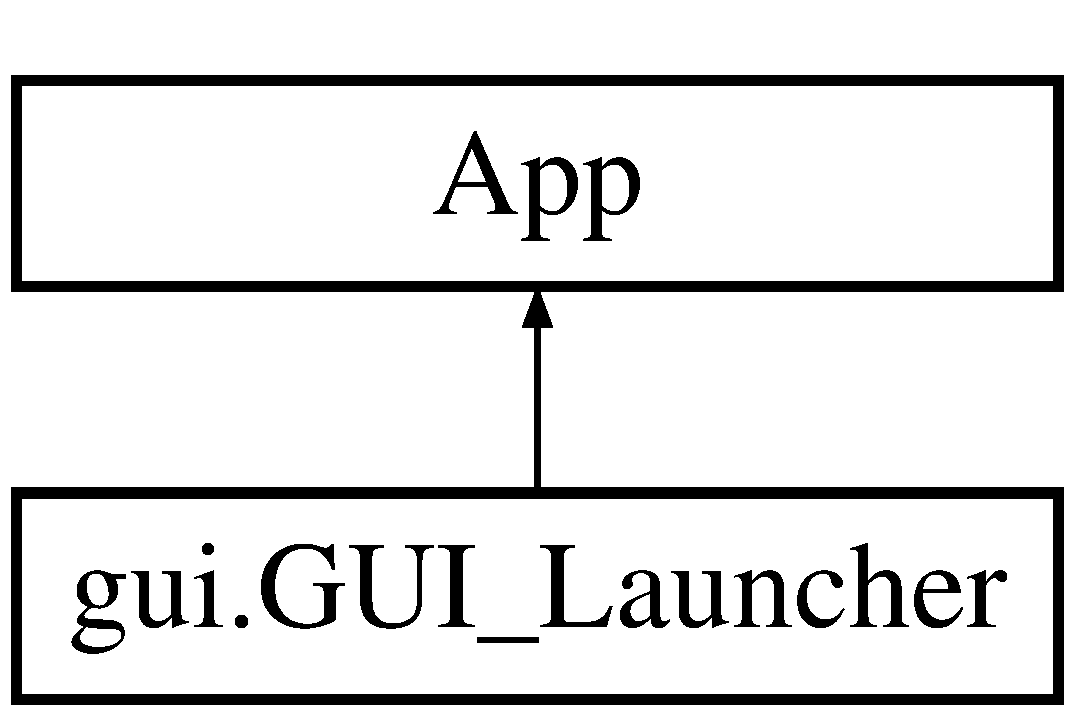
\includegraphics[height=2.000000cm]{classgui_1_1_g_u_i___launcher}
\end{center}
\end{figure}
\subsection*{Public Member Functions}
\begin{DoxyCompactItemize}
\item 
\hypertarget{classgui_1_1_g_u_i___launcher_a7ea6192bf60d4c6ed780d05859ad3682}{def \hyperlink{classgui_1_1_g_u_i___launcher_a7ea6192bf60d4c6ed780d05859ad3682}{On\-Init}}\label{classgui_1_1_g_u_i___launcher_a7ea6192bf60d4c6ed780d05859ad3682}

\begin{DoxyCompactList}\small\item\em Constuctor for a wx\-Python app. \end{DoxyCompactList}\end{DoxyCompactItemize}


\subsection{Detailed Description}
Abstracts away the creation of the \hyperlink{classgui_1_1_motor_g_u_i}{Motor\-G\-U\-I} and launches it in the default constructor. 

The documentation for this class was generated from the following file\-:\begin{DoxyCompactItemize}
\item 
gui.\-py\end{DoxyCompactItemize}

\hypertarget{classgui_1_1_motor_g_u_i}{\section{gui.\-Motor\-G\-U\-I Class Reference}
\label{classgui_1_1_motor_g_u_i}\index{gui.\-Motor\-G\-U\-I@{gui.\-Motor\-G\-U\-I}}
}


Defines the main frame for the G\-U\-I.  


Inheritance diagram for gui.\-Motor\-G\-U\-I\-:\begin{figure}[H]
\begin{center}
\leavevmode
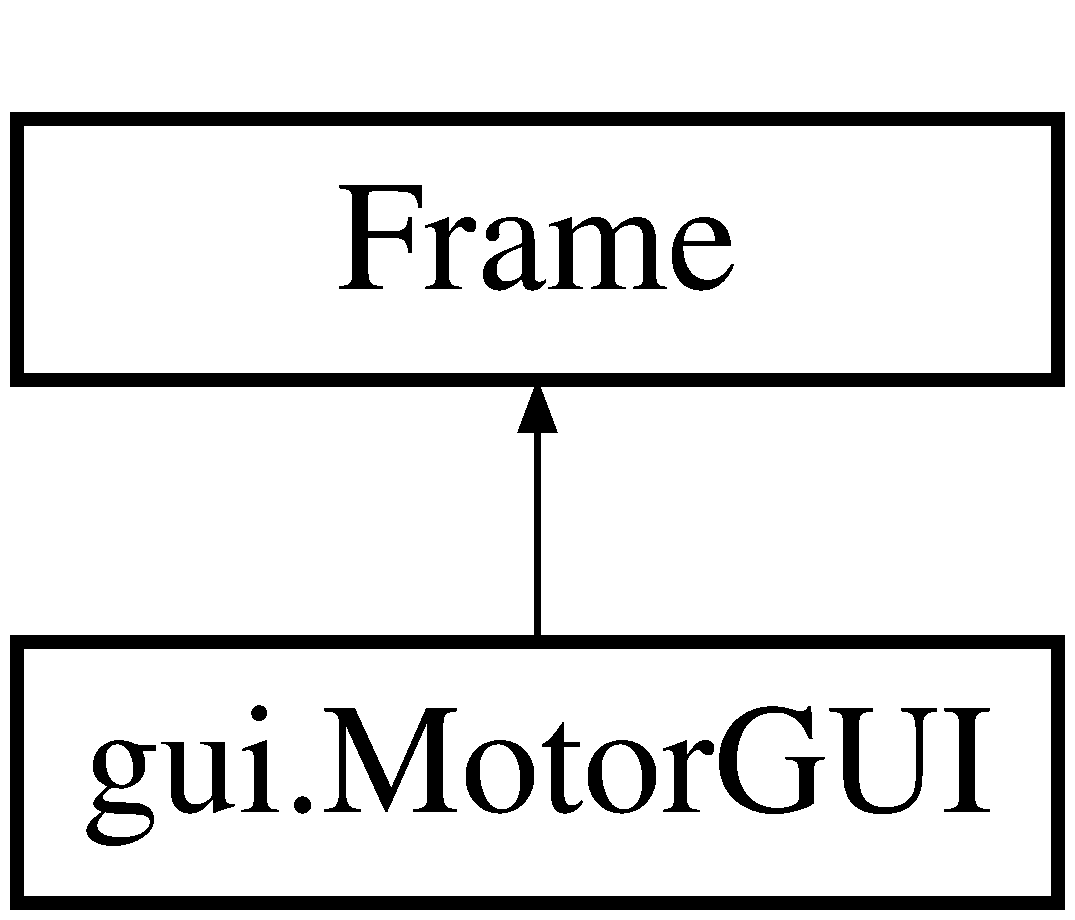
\includegraphics[height=2.000000cm]{classgui_1_1_motor_g_u_i}
\end{center}
\end{figure}
\subsection*{Public Member Functions}
\begin{DoxyCompactItemize}
\item 
\hypertarget{classgui_1_1_motor_g_u_i_a6095ad89d64af1d0b609562c63f7dc44}{def \hyperlink{classgui_1_1_motor_g_u_i_a6095ad89d64af1d0b609562c63f7dc44}{\-\_\-\-\_\-init\-\_\-\-\_\-}}\label{classgui_1_1_motor_g_u_i_a6095ad89d64af1d0b609562c63f7dc44}

\begin{DoxyCompactList}\small\item\em Constructor for a wx\-Python frame. \end{DoxyCompactList}\item 
def \hyperlink{classgui_1_1_motor_g_u_i_aa2d8e9800cfcf3bb0accbe3df3888216}{Start\-Update\-Thread}
\begin{DoxyCompactList}\small\item\em Initiates the thread that polls the Tiny for the value of the solar panel A\-D\-C and then updates the G\-U\-I accordingly. \end{DoxyCompactList}\item 
def \hyperlink{classgui_1_1_motor_g_u_i_a9a90f269ce5de4d5c2f234db8f984f02}{On\-Move\-Servo\-Request}
\begin{DoxyCompactList}\small\item\em Handles the event that is fired when the \char`\"{}\-Move Servo\char`\"{} button is pressed. \end{DoxyCompactList}\item 
def \hyperlink{classgui_1_1_motor_g_u_i_ac294c32d1139676f6adf61ccfcfdf07b}{On\-Solar\-Max\-Request}
\begin{DoxyCompactList}\small\item\em Handles the event that is fired when the \char`\"{}\-Maximize Solar Efficiency\char`\"{} button is pressed. \end{DoxyCompactList}\item 
def \hyperlink{classgui_1_1_motor_g_u_i_a387eaf79ea5f14461681d85559c6cc0d}{On\-Button\-Pressed}
\begin{DoxyCompactList}\small\item\em Handles the event that is fired when the \char`\"{}\-Connect\char`\"{} button is pressed. \end{DoxyCompactList}\item 
def \hyperlink{classgui_1_1_motor_g_u_i_a00bd7d29278fdd47773be526bd020bb1}{On\-Window\-Closed}
\begin{DoxyCompactList}\small\item\em Handles the event that is called when the program is closed. \end{DoxyCompactList}\item 
def \hyperlink{classgui_1_1_motor_g_u_i_a65167987294a1780a28b483821334fda}{On\-Solar\-Measure\-Update}
\begin{DoxyCompactList}\small\item\em Handles the event that is called when a new A\-D\-C measurment from the solar panel connected to the tiny is received. \end{DoxyCompactList}\item 
def \hyperlink{classgui_1_1_motor_g_u_i_af8d32eaef13c8826b0e07f7f4154ff10}{On\-About\-Requested}
\begin{DoxyCompactList}\small\item\em Handles the event that is called when the about menu button is pressed. \end{DoxyCompactList}\end{DoxyCompactItemize}
\subsection*{Public Attributes}
\begin{DoxyCompactItemize}
\item 
\hypertarget{classgui_1_1_motor_g_u_i_a92a05554565e2d7939459090a17c50d6}{\hyperlink{classgui_1_1_motor_g_u_i_a92a05554565e2d7939459090a17c50d6}{solar\-\_\-event}}\label{classgui_1_1_motor_g_u_i_a92a05554565e2d7939459090a17c50d6}

\begin{DoxyCompactList}\small\item\em Holds the event type definition for the event that is called when the G\-U\-I needs to be updated with the latest solar panel measurement. \end{DoxyCompactList}\item 
\hypertarget{classgui_1_1_motor_g_u_i_af9222ac373f1bf876de393043a37a14c}{\hyperlink{classgui_1_1_motor_g_u_i_af9222ac373f1bf876de393043a37a14c}{usb}}\label{classgui_1_1_motor_g_u_i_af9222ac373f1bf876de393043a37a14c}

\begin{DoxyCompactList}\small\item\em Holds the usb connection variable that is used to interface with the Tiny261. \end{DoxyCompactList}\item 
\hypertarget{classgui_1_1_motor_g_u_i_a077928e387639fcff3f7ce1067090c78}{\hyperlink{classgui_1_1_motor_g_u_i_a077928e387639fcff3f7ce1067090c78}{connect}}\label{classgui_1_1_motor_g_u_i_a077928e387639fcff3f7ce1067090c78}

\begin{DoxyCompactList}\small\item\em The \char`\"{}\-Connect\char`\"{} button. \end{DoxyCompactList}\item 
\hypertarget{classgui_1_1_motor_g_u_i_ab7c6435d9f97f47d48dea18161533474}{\hyperlink{classgui_1_1_motor_g_u_i_ab7c6435d9f97f47d48dea18161533474}{find\-\_\-sun}}\label{classgui_1_1_motor_g_u_i_ab7c6435d9f97f47d48dea18161533474}

\begin{DoxyCompactList}\small\item\em The \char`\"{}\-Maximize Solar Efficiency\char`\"{} button. \end{DoxyCompactList}\item 
\hyperlink{classgui_1_1_motor_g_u_i_acfe4b83245af20371a2c71e8997f8139}{position}
\begin{DoxyCompactList}\small\item\em The \char`\"{}\-Position\char`\"{} text control (allows the user to specifiy a position to move the servo). \end{DoxyCompactList}\item 
\hyperlink{classgui_1_1_motor_g_u_i_adcbde7aacf6312ceff8d675cc27b40fa}{display}
\begin{DoxyCompactList}\small\item\em The \char`\"{}\-Display\char`\"{} text control (shows the solar panel measurements). \end{DoxyCompactList}\item 
\hyperlink{classgui_1_1_motor_g_u_i_a142d48a338fab59d090ceb50e9e01748}{move}
\begin{DoxyCompactList}\small\item\em The \char`\"{}\-Move Servo\char`\"{} button. \end{DoxyCompactList}\item 
\hyperlink{classgui_1_1_motor_g_u_i_ab0f241eaebfd0d70b12982ad52f8ea33}{gauge}
\begin{DoxyCompactList}\small\item\em The solar measurements Gauge (displays the measurements in gauge form). \end{DoxyCompactList}\item 
\hypertarget{classgui_1_1_motor_g_u_i_ad575070f85c5265bf2b2607aab5236fe}{\hyperlink{classgui_1_1_motor_g_u_i_ad575070f85c5265bf2b2607aab5236fe}{updater}}\label{classgui_1_1_motor_g_u_i_ad575070f85c5265bf2b2607aab5236fe}

\begin{DoxyCompactList}\small\item\em Holds the object that corresponds to the solar panel measurements update thread. \end{DoxyCompactList}\end{DoxyCompactItemize}


\subsection{Detailed Description}
Defines the main frame for the G\-U\-I. 

It provides a simple interface for the user to send commands to a Tiny261 microcontroller (that has the approriate firmware) via the O\-S\-Uisp2 Universal Programmer. The commands move a solar panel to certain positions and take measurements that correspond to the amount of light that is hitting the solar panel. Those measurements are echoed back to the computer, which are displayed on the G\-U\-I. 

\subsection{Member Function Documentation}
\hypertarget{classgui_1_1_motor_g_u_i_af8d32eaef13c8826b0e07f7f4154ff10}{\index{gui\-::\-Motor\-G\-U\-I@{gui\-::\-Motor\-G\-U\-I}!On\-About\-Requested@{On\-About\-Requested}}
\index{On\-About\-Requested@{On\-About\-Requested}!gui::MotorGUI@{gui\-::\-Motor\-G\-U\-I}}
\subsubsection[{On\-About\-Requested}]{\setlength{\rightskip}{0pt plus 5cm}def gui.\-Motor\-G\-U\-I.\-On\-About\-Requested (
\begin{DoxyParamCaption}
\item[{}]{self, }
\item[{}]{event}
\end{DoxyParamCaption}
)}}\label{classgui_1_1_motor_g_u_i_af8d32eaef13c8826b0e07f7f4154ff10}


Handles the event that is called when the about menu button is pressed. 

Shows the user a message box containing information about the program


\begin{DoxyParams}{Parameters}
{\em self,\-:} & The object pointer \\
\hline
{\em event,\-:} & The object that is associated with the event request \\
\hline
\end{DoxyParams}
\hypertarget{classgui_1_1_motor_g_u_i_a387eaf79ea5f14461681d85559c6cc0d}{\index{gui\-::\-Motor\-G\-U\-I@{gui\-::\-Motor\-G\-U\-I}!On\-Button\-Pressed@{On\-Button\-Pressed}}
\index{On\-Button\-Pressed@{On\-Button\-Pressed}!gui::MotorGUI@{gui\-::\-Motor\-G\-U\-I}}
\subsubsection[{On\-Button\-Pressed}]{\setlength{\rightskip}{0pt plus 5cm}def gui.\-Motor\-G\-U\-I.\-On\-Button\-Pressed (
\begin{DoxyParamCaption}
\item[{}]{self, }
\item[{}]{event}
\end{DoxyParamCaption}
)}}\label{classgui_1_1_motor_g_u_i_a387eaf79ea5f14461681d85559c6cc0d}


Handles the event that is fired when the \char`\"{}\-Connect\char`\"{} button is pressed. 

If a usb connection is not currently active, the G\-U\-I sends a request to the O\-S\-Uisp2 programmer to connect to the Tiny and verify that the correct firmware is installed.


\begin{DoxyParams}{Parameters}
{\em self,\-:} & The object pointer \\
\hline
{\em event,\-:} & The object that is associated with the event request \\
\hline
\end{DoxyParams}
\hypertarget{classgui_1_1_motor_g_u_i_a9a90f269ce5de4d5c2f234db8f984f02}{\index{gui\-::\-Motor\-G\-U\-I@{gui\-::\-Motor\-G\-U\-I}!On\-Move\-Servo\-Request@{On\-Move\-Servo\-Request}}
\index{On\-Move\-Servo\-Request@{On\-Move\-Servo\-Request}!gui::MotorGUI@{gui\-::\-Motor\-G\-U\-I}}
\subsubsection[{On\-Move\-Servo\-Request}]{\setlength{\rightskip}{0pt plus 5cm}def gui.\-Motor\-G\-U\-I.\-On\-Move\-Servo\-Request (
\begin{DoxyParamCaption}
\item[{}]{self, }
\item[{}]{event}
\end{DoxyParamCaption}
)}}\label{classgui_1_1_motor_g_u_i_a9a90f269ce5de4d5c2f234db8f984f02}


Handles the event that is fired when the \char`\"{}\-Move Servo\char`\"{} button is pressed. 

If a usb connection is currently active, a request is sent to the Tiny to move the motor to the position that corresponds to value given by the user in the position text control. The solar measurement update thread is paused until the Tiny26 is finished repositioning the motor


\begin{DoxyParams}{Parameters}
{\em self,\-:} & The object pointer \\
\hline
{\em event,\-:} & The object that is associated with the event request \\
\hline
\end{DoxyParams}
\hypertarget{classgui_1_1_motor_g_u_i_ac294c32d1139676f6adf61ccfcfdf07b}{\index{gui\-::\-Motor\-G\-U\-I@{gui\-::\-Motor\-G\-U\-I}!On\-Solar\-Max\-Request@{On\-Solar\-Max\-Request}}
\index{On\-Solar\-Max\-Request@{On\-Solar\-Max\-Request}!gui::MotorGUI@{gui\-::\-Motor\-G\-U\-I}}
\subsubsection[{On\-Solar\-Max\-Request}]{\setlength{\rightskip}{0pt plus 5cm}def gui.\-Motor\-G\-U\-I.\-On\-Solar\-Max\-Request (
\begin{DoxyParamCaption}
\item[{}]{self, }
\item[{}]{event}
\end{DoxyParamCaption}
)}}\label{classgui_1_1_motor_g_u_i_ac294c32d1139676f6adf61ccfcfdf07b}


Handles the event that is fired when the \char`\"{}\-Maximize Solar Efficiency\char`\"{} button is pressed. 

If a usb connection is currently active, a request to find the position that produces the highest voltage output from the solar panel is sent. The solar panel measurement update thread is paused until the Tiny had finished positioning the solar panel in the position that receives the most light.


\begin{DoxyParams}{Parameters}
{\em self,\-:} & The object pointer \\
\hline
{\em event,\-:} & The object that is associated with the event request \\
\hline
\end{DoxyParams}
\hypertarget{classgui_1_1_motor_g_u_i_a65167987294a1780a28b483821334fda}{\index{gui\-::\-Motor\-G\-U\-I@{gui\-::\-Motor\-G\-U\-I}!On\-Solar\-Measure\-Update@{On\-Solar\-Measure\-Update}}
\index{On\-Solar\-Measure\-Update@{On\-Solar\-Measure\-Update}!gui::MotorGUI@{gui\-::\-Motor\-G\-U\-I}}
\subsubsection[{On\-Solar\-Measure\-Update}]{\setlength{\rightskip}{0pt plus 5cm}def gui.\-Motor\-G\-U\-I.\-On\-Solar\-Measure\-Update (
\begin{DoxyParamCaption}
\item[{}]{self, }
\item[{}]{event}
\end{DoxyParamCaption}
)}}\label{classgui_1_1_motor_g_u_i_a65167987294a1780a28b483821334fda}


Handles the event that is called when a new A\-D\-C measurment from the solar panel connected to the tiny is received. 

Sets the value of the text control equal to the measurement that is contained in the event request.


\begin{DoxyParams}{Parameters}
{\em self,\-:} & The object pointer \\
\hline
{\em event,\-:} & The object that is associated with the event request \\
\hline
\end{DoxyParams}
\hypertarget{classgui_1_1_motor_g_u_i_a00bd7d29278fdd47773be526bd020bb1}{\index{gui\-::\-Motor\-G\-U\-I@{gui\-::\-Motor\-G\-U\-I}!On\-Window\-Closed@{On\-Window\-Closed}}
\index{On\-Window\-Closed@{On\-Window\-Closed}!gui::MotorGUI@{gui\-::\-Motor\-G\-U\-I}}
\subsubsection[{On\-Window\-Closed}]{\setlength{\rightskip}{0pt plus 5cm}def gui.\-Motor\-G\-U\-I.\-On\-Window\-Closed (
\begin{DoxyParamCaption}
\item[{}]{self, }
\item[{}]{event}
\end{DoxyParamCaption}
)}}\label{classgui_1_1_motor_g_u_i_a00bd7d29278fdd47773be526bd020bb1}


Handles the event that is called when the program is closed. 

If a usb connection is currently active, the G\-U\-I sends a request to the O\-S\-Uisp2 programmer to close the connection to the Tiny and to end the thread that updates the G\-U\-I with the solar panel measurments


\begin{DoxyParams}{Parameters}
{\em self,\-:} & The object pointer \\
\hline
{\em event,\-:} & The object that is associated with the event request \\
\hline
\end{DoxyParams}
\hypertarget{classgui_1_1_motor_g_u_i_aa2d8e9800cfcf3bb0accbe3df3888216}{\index{gui\-::\-Motor\-G\-U\-I@{gui\-::\-Motor\-G\-U\-I}!Start\-Update\-Thread@{Start\-Update\-Thread}}
\index{Start\-Update\-Thread@{Start\-Update\-Thread}!gui::MotorGUI@{gui\-::\-Motor\-G\-U\-I}}
\subsubsection[{Start\-Update\-Thread}]{\setlength{\rightskip}{0pt plus 5cm}def gui.\-Motor\-G\-U\-I.\-Start\-Update\-Thread (
\begin{DoxyParamCaption}
\item[{}]{self}
\end{DoxyParamCaption}
)}}\label{classgui_1_1_motor_g_u_i_aa2d8e9800cfcf3bb0accbe3df3888216}


Initiates the thread that polls the Tiny for the value of the solar panel A\-D\-C and then updates the G\-U\-I accordingly. 


\begin{DoxyParams}{Parameters}
{\em self,\-:} & The object pointer \\
\hline
\end{DoxyParams}


\subsection{Member Data Documentation}
\hypertarget{classgui_1_1_motor_g_u_i_adcbde7aacf6312ceff8d675cc27b40fa}{\index{gui\-::\-Motor\-G\-U\-I@{gui\-::\-Motor\-G\-U\-I}!display@{display}}
\index{display@{display}!gui::MotorGUI@{gui\-::\-Motor\-G\-U\-I}}
\subsubsection[{display}]{\setlength{\rightskip}{0pt plus 5cm}gui.\-Motor\-G\-U\-I.\-display}}\label{classgui_1_1_motor_g_u_i_adcbde7aacf6312ceff8d675cc27b40fa}


The \char`\"{}\-Display\char`\"{} text control (shows the solar panel measurements). 

\hypertarget{classgui_1_1_motor_g_u_i_ab0f241eaebfd0d70b12982ad52f8ea33}{\index{gui\-::\-Motor\-G\-U\-I@{gui\-::\-Motor\-G\-U\-I}!gauge@{gauge}}
\index{gauge@{gauge}!gui::MotorGUI@{gui\-::\-Motor\-G\-U\-I}}
\subsubsection[{gauge}]{\setlength{\rightskip}{0pt plus 5cm}gui.\-Motor\-G\-U\-I.\-gauge}}\label{classgui_1_1_motor_g_u_i_ab0f241eaebfd0d70b12982ad52f8ea33}


The solar measurements Gauge (displays the measurements in gauge form). 

\hypertarget{classgui_1_1_motor_g_u_i_a142d48a338fab59d090ceb50e9e01748}{\index{gui\-::\-Motor\-G\-U\-I@{gui\-::\-Motor\-G\-U\-I}!move@{move}}
\index{move@{move}!gui::MotorGUI@{gui\-::\-Motor\-G\-U\-I}}
\subsubsection[{move}]{\setlength{\rightskip}{0pt plus 5cm}gui.\-Motor\-G\-U\-I.\-move}}\label{classgui_1_1_motor_g_u_i_a142d48a338fab59d090ceb50e9e01748}


The \char`\"{}\-Move Servo\char`\"{} button. 

\hypertarget{classgui_1_1_motor_g_u_i_acfe4b83245af20371a2c71e8997f8139}{\index{gui\-::\-Motor\-G\-U\-I@{gui\-::\-Motor\-G\-U\-I}!position@{position}}
\index{position@{position}!gui::MotorGUI@{gui\-::\-Motor\-G\-U\-I}}
\subsubsection[{position}]{\setlength{\rightskip}{0pt plus 5cm}gui.\-Motor\-G\-U\-I.\-position}}\label{classgui_1_1_motor_g_u_i_acfe4b83245af20371a2c71e8997f8139}


The \char`\"{}\-Position\char`\"{} text control (allows the user to specifiy a position to move the servo). 



The documentation for this class was generated from the following file\-:\begin{DoxyCompactItemize}
\item 
gui.\-py\end{DoxyCompactItemize}

\hypertarget{classtiny26_1_1_solar_event}{\section{tiny26.\-Solar\-Event Class Reference}
\label{classtiny26_1_1_solar_event}\index{tiny26.\-Solar\-Event@{tiny26.\-Solar\-Event}}
}


Event class that allows a background thread to send messages to G\-U\-I to tell it to update itself.  


Inheritance diagram for tiny26.\-Solar\-Event\-:\begin{figure}[H]
\begin{center}
\leavevmode
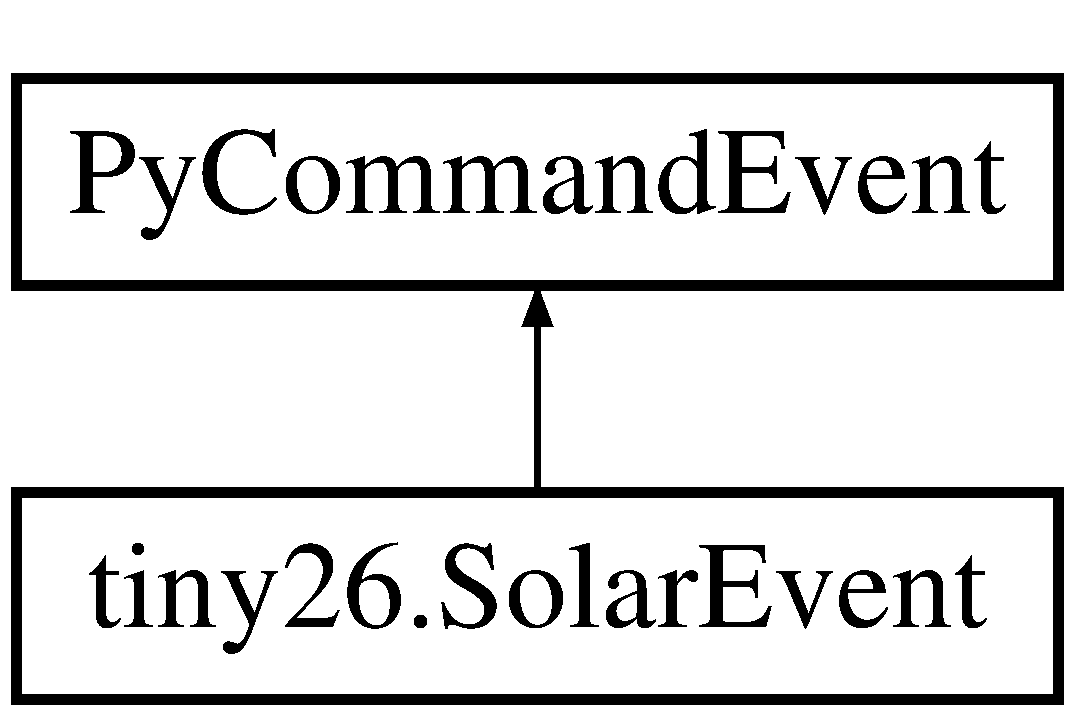
\includegraphics[height=2.000000cm]{classtiny26_1_1_solar_event}
\end{center}
\end{figure}
\subsection*{Public Member Functions}
\begin{DoxyCompactItemize}
\item 
\hypertarget{classtiny26_1_1_solar_event_aeda315c23993c95cb7df7361f88ba4ec}{def \hyperlink{classtiny26_1_1_solar_event_aeda315c23993c95cb7df7361f88ba4ec}{\-\_\-\-\_\-init\-\_\-\-\_\-}}\label{classtiny26_1_1_solar_event_aeda315c23993c95cb7df7361f88ba4ec}

\begin{DoxyCompactList}\small\item\em Constructor for the solar event. \end{DoxyCompactList}\item 
def \hyperlink{classtiny26_1_1_solar_event_a0d404d7b007e93b998a57f1bad88dcac}{Get\-Value}
\begin{DoxyCompactList}\small\item\em Returns the value of the event that is set in the constructor. \end{DoxyCompactList}\end{DoxyCompactItemize}


\subsection{Detailed Description}
Event class that allows a background thread to send messages to G\-U\-I to tell it to update itself. 

\subsection{Member Function Documentation}
\hypertarget{classtiny26_1_1_solar_event_a0d404d7b007e93b998a57f1bad88dcac}{\index{tiny26\-::\-Solar\-Event@{tiny26\-::\-Solar\-Event}!Get\-Value@{Get\-Value}}
\index{Get\-Value@{Get\-Value}!tiny26::SolarEvent@{tiny26\-::\-Solar\-Event}}
\subsubsection[{Get\-Value}]{\setlength{\rightskip}{0pt plus 5cm}def tiny26.\-Solar\-Event.\-Get\-Value (
\begin{DoxyParamCaption}
\item[{}]{self}
\end{DoxyParamCaption}
)}}\label{classtiny26_1_1_solar_event_a0d404d7b007e93b998a57f1bad88dcac}


Returns the value of the event that is set in the constructor. 


\begin{DoxyParams}{Parameters}
{\em self,\-:} & The object pointer \\
\hline
\end{DoxyParams}


The documentation for this class was generated from the following file\-:\begin{DoxyCompactItemize}
\item 
tiny26.\-py\end{DoxyCompactItemize}

\hypertarget{classtiny26_1_1_solar_tracking_thread}{\section{tiny26.\-Solar\-Tracking\-Thread Class Reference}
\label{classtiny26_1_1_solar_tracking_thread}\index{tiny26.\-Solar\-Tracking\-Thread@{tiny26.\-Solar\-Tracking\-Thread}}
}


Contains the definition for the background thread that polls the A\-D\-C input from the solar panel and sends that value to the G\-U\-I to be displayed to the user.  


Inheritance diagram for tiny26.\-Solar\-Tracking\-Thread\-:\begin{figure}[H]
\begin{center}
\leavevmode
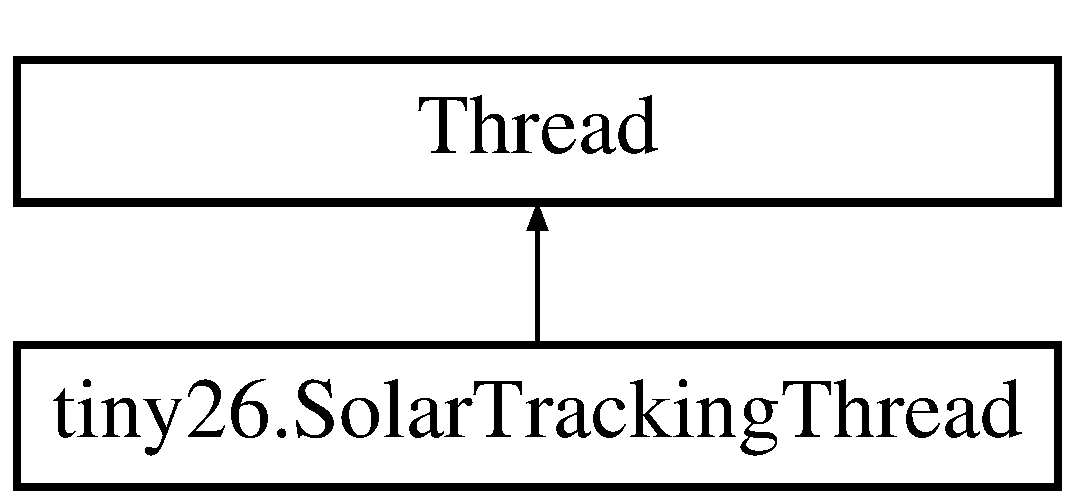
\includegraphics[height=2.000000cm]{classtiny26_1_1_solar_tracking_thread}
\end{center}
\end{figure}
\subsection*{Public Member Functions}
\begin{DoxyCompactItemize}
\item 
\hypertarget{classtiny26_1_1_solar_tracking_thread_a4c08b8abae1040b50dcd96f8f2386e40}{def \hyperlink{classtiny26_1_1_solar_tracking_thread_a4c08b8abae1040b50dcd96f8f2386e40}{\-\_\-\-\_\-init\-\_\-\-\_\-}}\label{classtiny26_1_1_solar_tracking_thread_a4c08b8abae1040b50dcd96f8f2386e40}

\begin{DoxyCompactList}\small\item\em Constructor for the solar tracking thread. \end{DoxyCompactList}\item 
def \hyperlink{classtiny26_1_1_solar_tracking_thread_a006529500ed94214eef1c856cc6cbc5b}{run}
\begin{DoxyCompactList}\small\item\em Called when the thread is started. \end{DoxyCompactList}\item 
def \hyperlink{classtiny26_1_1_solar_tracking_thread_a068e98629f1f0a139914e4d7a41d134b}{Quit\-Thread}
\begin{DoxyCompactList}\small\item\em Sets the stop flag to stop the thread. \end{DoxyCompactList}\end{DoxyCompactItemize}
\subsection*{Public Attributes}
\begin{DoxyCompactItemize}
\item 
\hypertarget{classtiny26_1_1_solar_tracking_thread_a4b7452fd152929e399adf0e263c6e472}{\hyperlink{classtiny26_1_1_solar_tracking_thread_a4b7452fd152929e399adf0e263c6e472}{usb}}\label{classtiny26_1_1_solar_tracking_thread_a4b7452fd152929e399adf0e263c6e472}

\begin{DoxyCompactList}\small\item\em The usb interface associated with the thread. \end{DoxyCompactList}\item 
\hypertarget{classtiny26_1_1_solar_tracking_thread_a806015811adc26b8af26f48ce2c1de78}{\hyperlink{classtiny26_1_1_solar_tracking_thread_a806015811adc26b8af26f48ce2c1de78}{event}}\label{classtiny26_1_1_solar_tracking_thread_a806015811adc26b8af26f48ce2c1de78}

\begin{DoxyCompactList}\small\item\em The event that needs to be fired when the G\-U\-I needs to be updated. \end{DoxyCompactList}\item 
\hypertarget{classtiny26_1_1_solar_tracking_thread_a96bd262571f5cefa8f5fcb05256745cb}{\hyperlink{classtiny26_1_1_solar_tracking_thread_a96bd262571f5cefa8f5fcb05256745cb}{parent}}\label{classtiny26_1_1_solar_tracking_thread_a96bd262571f5cefa8f5fcb05256745cb}

\begin{DoxyCompactList}\small\item\em The parent frame that should be updated when a new solar measurement is received. \end{DoxyCompactList}\item 
\hypertarget{classtiny26_1_1_solar_tracking_thread_a03b6d1de5dd4ebf8d64450d248ad0fe9}{\hyperlink{classtiny26_1_1_solar_tracking_thread_a03b6d1de5dd4ebf8d64450d248ad0fe9}{stop}}\label{classtiny26_1_1_solar_tracking_thread_a03b6d1de5dd4ebf8d64450d248ad0fe9}

\begin{DoxyCompactList}\small\item\em The stop flag for the thread. \end{DoxyCompactList}\end{DoxyCompactItemize}


\subsection{Detailed Description}
Contains the definition for the background thread that polls the A\-D\-C input from the solar panel and sends that value to the G\-U\-I to be displayed to the user. 

\subsection{Member Function Documentation}
\hypertarget{classtiny26_1_1_solar_tracking_thread_a068e98629f1f0a139914e4d7a41d134b}{\index{tiny26\-::\-Solar\-Tracking\-Thread@{tiny26\-::\-Solar\-Tracking\-Thread}!Quit\-Thread@{Quit\-Thread}}
\index{Quit\-Thread@{Quit\-Thread}!tiny26::SolarTrackingThread@{tiny26\-::\-Solar\-Tracking\-Thread}}
\subsubsection[{Quit\-Thread}]{\setlength{\rightskip}{0pt plus 5cm}def tiny26.\-Solar\-Tracking\-Thread.\-Quit\-Thread (
\begin{DoxyParamCaption}
\item[{}]{self}
\end{DoxyParamCaption}
)}}\label{classtiny26_1_1_solar_tracking_thread_a068e98629f1f0a139914e4d7a41d134b}


Sets the stop flag to stop the thread. 

Sets the stop flag, which causes the loop in the thread to stop if it was running


\begin{DoxyParams}{Parameters}
{\em self,\-:} & The object pointer \\
\hline
\end{DoxyParams}
\hypertarget{classtiny26_1_1_solar_tracking_thread_a006529500ed94214eef1c856cc6cbc5b}{\index{tiny26\-::\-Solar\-Tracking\-Thread@{tiny26\-::\-Solar\-Tracking\-Thread}!run@{run}}
\index{run@{run}!tiny26::SolarTrackingThread@{tiny26\-::\-Solar\-Tracking\-Thread}}
\subsubsection[{run}]{\setlength{\rightskip}{0pt plus 5cm}def tiny26.\-Solar\-Tracking\-Thread.\-run (
\begin{DoxyParamCaption}
\item[{}]{self}
\end{DoxyParamCaption}
)}}\label{classtiny26_1_1_solar_tracking_thread_a006529500ed94214eef1c856cc6cbc5b}


Called when the thread is started. 

As long as the stop flag is not set, the thread sends a request to the Tiny for solar measurements. When the computer receives a response from the Tiny, it fires a \hyperlink{classtiny26_1_1_solar_event}{Solar\-Event}, which tells the G\-U\-I to update itself with the latest solar measurements.


\begin{DoxyParams}{Parameters}
{\em self,\-:} & The object pointer \\
\hline
\end{DoxyParams}


The documentation for this class was generated from the following file\-:\begin{DoxyCompactItemize}
\item 
tiny26.\-py\end{DoxyCompactItemize}

\hypertarget{classtiny26_1_1_u_s_b___interface}{\section{tiny26.\-U\-S\-B\-\_\-\-Interface Class Reference}
\label{classtiny26_1_1_u_s_b___interface}\index{tiny26.\-U\-S\-B\-\_\-\-Interface@{tiny26.\-U\-S\-B\-\_\-\-Interface}}
}


The usb interface for the O\-S\-Uisp2 and the Tiny261 is contained in this class.  


\subsection*{Public Member Functions}
\begin{DoxyCompactItemize}
\item 
\hypertarget{classtiny26_1_1_u_s_b___interface_a7f215a18e8b642c3fbdd85034341bfec}{def \hyperlink{classtiny26_1_1_u_s_b___interface_a7f215a18e8b642c3fbdd85034341bfec}{\-\_\-\-\_\-init\-\_\-\-\_\-}}\label{classtiny26_1_1_u_s_b___interface_a7f215a18e8b642c3fbdd85034341bfec}

\begin{DoxyCompactList}\small\item\em Constructor for the usb interface. \end{DoxyCompactList}\item 
def \hyperlink{classtiny26_1_1_u_s_b___interface_a4253137584b496ee45353b5a3c061bfb}{Is\-Connected}
\begin{DoxyCompactList}\small\item\em Returns the connection status. \end{DoxyCompactList}\item 
def \hyperlink{classtiny26_1_1_u_s_b___interface_a77bb39d15835e15e5ff0dcfc1de4bbda}{Measure\-Solar\-Panel}
\begin{DoxyCompactList}\small\item\em Reads the output of the solar panel. \end{DoxyCompactList}\item 
def \hyperlink{classtiny26_1_1_u_s_b___interface_aafc201d921ed8e71f6068f130e47b5e9}{Find\-Most\-Sun}
\begin{DoxyCompactList}\small\item\em Moves the solar panel to its optimal position. \end{DoxyCompactList}\item 
def \hyperlink{classtiny26_1_1_u_s_b___interface_ad469c3dcb16971e83b5f6827999da033}{Set\-Solar\-Position}
\begin{DoxyCompactList}\small\item\em Moves the solar panel to the specified position. \end{DoxyCompactList}\item 
def \hyperlink{classtiny26_1_1_u_s_b___interface_a2b0699d9fc55586245706cf07fb2361c}{Show\-Error\-Msg}
\begin{DoxyCompactList}\small\item\em Displays an error message box with the supplied message and title. \end{DoxyCompactList}\item 
def \hyperlink{classtiny26_1_1_u_s_b___interface_af674dcd1942eb31f15280d41b5f0e4d3}{Close\-Connection}
\begin{DoxyCompactList}\small\item\em Cleans up the connection to the Tiny26. \end{DoxyCompactList}\end{DoxyCompactItemize}
\subsection*{Public Attributes}
\begin{DoxyCompactItemize}
\item 
\hypertarget{classtiny26_1_1_u_s_b___interface_a52e6b805c40277c871717f365de8dd16}{\hyperlink{classtiny26_1_1_u_s_b___interface_a52e6b805c40277c871717f365de8dd16}{window}}\label{classtiny26_1_1_u_s_b___interface_a52e6b805c40277c871717f365de8dd16}

\begin{DoxyCompactList}\small\item\em The frame that is associated with the U\-S\-B interface. \end{DoxyCompactList}\item 
\hypertarget{classtiny26_1_1_u_s_b___interface_a2625b065c6150108c013f35773de24f2}{\hyperlink{classtiny26_1_1_u_s_b___interface_a2625b065c6150108c013f35773de24f2}{lib}}\label{classtiny26_1_1_u_s_b___interface_a2625b065c6150108c013f35773de24f2}

\begin{DoxyCompactList}\small\item\em tiny26usb.\-dll library \end{DoxyCompactList}\item 
\hypertarget{classtiny26_1_1_u_s_b___interface_a41e15534c462ecca4c4df61572e4b9ee}{\hyperlink{classtiny26_1_1_u_s_b___interface_a41e15534c462ecca4c4df61572e4b9ee}{device}}\label{classtiny26_1_1_u_s_b___interface_a41e15534c462ecca4c4df61572e4b9ee}

\begin{DoxyCompactList}\small\item\em usb\-Device\-\_\-t $\ast$ needed to establish a connection with O\-S\-Uisp2 and the Tiny \end{DoxyCompactList}\item 
\hypertarget{classtiny26_1_1_u_s_b___interface_ae04d38cc27318c29dd28bd3ee4c28e96}{\hyperlink{classtiny26_1_1_u_s_b___interface_ae04d38cc27318c29dd28bd3ee4c28e96}{connected}}\label{classtiny26_1_1_u_s_b___interface_ae04d38cc27318c29dd28bd3ee4c28e96}

\begin{DoxyCompactList}\small\item\em Holds the connection status. \end{DoxyCompactList}\end{DoxyCompactItemize}


\subsection{Detailed Description}
The usb interface for the O\-S\-Uisp2 and the Tiny261 is contained in this class. 

It contains all the methods for establishing connections, closing connections, and sending request to the Tiny261 to move the servo and to get the A\-D\-C measurements from the solar panel. 

\subsection{Member Function Documentation}
\hypertarget{classtiny26_1_1_u_s_b___interface_af674dcd1942eb31f15280d41b5f0e4d3}{\index{tiny26\-::\-U\-S\-B\-\_\-\-Interface@{tiny26\-::\-U\-S\-B\-\_\-\-Interface}!Close\-Connection@{Close\-Connection}}
\index{Close\-Connection@{Close\-Connection}!tiny26::USB_Interface@{tiny26\-::\-U\-S\-B\-\_\-\-Interface}}
\subsubsection[{Close\-Connection}]{\setlength{\rightskip}{0pt plus 5cm}def tiny26.\-U\-S\-B\-\_\-\-Interface.\-Close\-Connection (
\begin{DoxyParamCaption}
\item[{}]{self}
\end{DoxyParamCaption}
)}}\label{classtiny26_1_1_u_s_b___interface_af674dcd1942eb31f15280d41b5f0e4d3}


Cleans up the connection to the Tiny26. 

Sends a request to the O\-S\-Uisp2 Universal Programmer to disconnect from the Tiny


\begin{DoxyParams}{Parameters}
{\em self,\-:} & The object pointer \\
\hline
\end{DoxyParams}
\hypertarget{classtiny26_1_1_u_s_b___interface_aafc201d921ed8e71f6068f130e47b5e9}{\index{tiny26\-::\-U\-S\-B\-\_\-\-Interface@{tiny26\-::\-U\-S\-B\-\_\-\-Interface}!Find\-Most\-Sun@{Find\-Most\-Sun}}
\index{Find\-Most\-Sun@{Find\-Most\-Sun}!tiny26::USB_Interface@{tiny26\-::\-U\-S\-B\-\_\-\-Interface}}
\subsubsection[{Find\-Most\-Sun}]{\setlength{\rightskip}{0pt plus 5cm}def tiny26.\-U\-S\-B\-\_\-\-Interface.\-Find\-Most\-Sun (
\begin{DoxyParamCaption}
\item[{}]{self}
\end{DoxyParamCaption}
)}}\label{classtiny26_1_1_u_s_b___interface_aafc201d921ed8e71f6068f130e47b5e9}


Moves the solar panel to its optimal position. 

Sends a request to the Tiny to search for the position that gives the solar panel the most light. The Tiny does not respond to any movement requests while it is searching for the solar panel's optimal position


\begin{DoxyParams}{Parameters}
{\em self,\-:} & The object pointer \\
\hline
\end{DoxyParams}
\hypertarget{classtiny26_1_1_u_s_b___interface_a4253137584b496ee45353b5a3c061bfb}{\index{tiny26\-::\-U\-S\-B\-\_\-\-Interface@{tiny26\-::\-U\-S\-B\-\_\-\-Interface}!Is\-Connected@{Is\-Connected}}
\index{Is\-Connected@{Is\-Connected}!tiny26::USB_Interface@{tiny26\-::\-U\-S\-B\-\_\-\-Interface}}
\subsubsection[{Is\-Connected}]{\setlength{\rightskip}{0pt plus 5cm}def tiny26.\-U\-S\-B\-\_\-\-Interface.\-Is\-Connected (
\begin{DoxyParamCaption}
\item[{}]{self}
\end{DoxyParamCaption}
)}}\label{classtiny26_1_1_u_s_b___interface_a4253137584b496ee45353b5a3c061bfb}


Returns the connection status. 


\begin{DoxyParams}{Parameters}
{\em self,\-:} & The object pointer \\
\hline
\end{DoxyParams}
\hypertarget{classtiny26_1_1_u_s_b___interface_a77bb39d15835e15e5ff0dcfc1de4bbda}{\index{tiny26\-::\-U\-S\-B\-\_\-\-Interface@{tiny26\-::\-U\-S\-B\-\_\-\-Interface}!Measure\-Solar\-Panel@{Measure\-Solar\-Panel}}
\index{Measure\-Solar\-Panel@{Measure\-Solar\-Panel}!tiny26::USB_Interface@{tiny26\-::\-U\-S\-B\-\_\-\-Interface}}
\subsubsection[{Measure\-Solar\-Panel}]{\setlength{\rightskip}{0pt plus 5cm}def tiny26.\-U\-S\-B\-\_\-\-Interface.\-Measure\-Solar\-Panel (
\begin{DoxyParamCaption}
\item[{}]{self}
\end{DoxyParamCaption}
)}}\label{classtiny26_1_1_u_s_b___interface_a77bb39d15835e15e5ff0dcfc1de4bbda}


Reads the output of the solar panel. 

Sends a request to the Tiny to keep the motor in the current position respond with the light measurements


\begin{DoxyParams}{Parameters}
{\em self,\-:} & The object pointer \\
\hline
\end{DoxyParams}
\hypertarget{classtiny26_1_1_u_s_b___interface_ad469c3dcb16971e83b5f6827999da033}{\index{tiny26\-::\-U\-S\-B\-\_\-\-Interface@{tiny26\-::\-U\-S\-B\-\_\-\-Interface}!Set\-Solar\-Position@{Set\-Solar\-Position}}
\index{Set\-Solar\-Position@{Set\-Solar\-Position}!tiny26::USB_Interface@{tiny26\-::\-U\-S\-B\-\_\-\-Interface}}
\subsubsection[{Set\-Solar\-Position}]{\setlength{\rightskip}{0pt plus 5cm}def tiny26.\-U\-S\-B\-\_\-\-Interface.\-Set\-Solar\-Position (
\begin{DoxyParamCaption}
\item[{}]{self, }
\item[{}]{position}
\end{DoxyParamCaption}
)}}\label{classtiny26_1_1_u_s_b___interface_ad469c3dcb16971e83b5f6827999da033}


Moves the solar panel to the specified position. 

Sends a request to the Tiny to move the servo to the specified position. The Tiny will not respond to any requests while it is moving the servo. If the given position is out of the valid range, the servo moves to 254 or 1 depending on which extrema was violated


\begin{DoxyParams}{Parameters}
{\em self,\-:} & The object pointer \\
\hline
{\em position,\-:} & The desired position (0 $<$ position $<$ 255) \\
\hline
\end{DoxyParams}
\hypertarget{classtiny26_1_1_u_s_b___interface_a2b0699d9fc55586245706cf07fb2361c}{\index{tiny26\-::\-U\-S\-B\-\_\-\-Interface@{tiny26\-::\-U\-S\-B\-\_\-\-Interface}!Show\-Error\-Msg@{Show\-Error\-Msg}}
\index{Show\-Error\-Msg@{Show\-Error\-Msg}!tiny26::USB_Interface@{tiny26\-::\-U\-S\-B\-\_\-\-Interface}}
\subsubsection[{Show\-Error\-Msg}]{\setlength{\rightskip}{0pt plus 5cm}def tiny26.\-U\-S\-B\-\_\-\-Interface.\-Show\-Error\-Msg (
\begin{DoxyParamCaption}
\item[{}]{self, }
\item[{}]{message, }
\item[{}]{title}
\end{DoxyParamCaption}
)}}\label{classtiny26_1_1_u_s_b___interface_a2b0699d9fc55586245706cf07fb2361c}


Displays an error message box with the supplied message and title. 


\begin{DoxyParams}{Parameters}
{\em self,\-:} & The object pointer \\
\hline
{\em message,\-:} & The desired message for the Message Box \\
\hline
{\em title,\-:} & The desired title for the Message Box \\
\hline
\end{DoxyParams}


The documentation for this class was generated from the following file\-:\begin{DoxyCompactItemize}
\item 
tiny26.\-py\end{DoxyCompactItemize}

\addcontentsline{toc}{part}{Index}
\printindex
\end{document}
